\chapter{StyleGAN}
\begin{onehalfspace}
    In past, most improvement has been made to discriminator models in an effort to train more effective generator models, although less effort has been put into improving the generator models. The Style Generative Adversarial Network, or StyleGAN for short, is an extension to the GAN architecture that proposes large changes to the generator model, including the use of a mapping network to map points in latent space to an intermediate latent space, the use of the intermediate latent space to control style at each point in the generator model, and the introduction to noise as a source of variation at each point in the generator model. The resulting model is capable not only of generating impressively photorealistic high-quality photos of faces, but also offers control over the style of the generated image at different levels of detail through varying the style vectors and noise.
\section{Lacking Control Over Synthesized Images}
    Generative adversarial networks are effective at generating high-quality and large-resolution synthetic images. Many improvements to the GAN architecture have been achieved through enhancements to the discriminator model. These changes are motivated by the idea that a better discriminator model will, in turn, lead to the generation of more realistic synthetic images. As such, the generator has been somewhat neglected and remains a black box. This limited understanding of the generator is perhaps most exemplified by the general lack of control over the generated images. There are few tools to control the properties of generated images, e.g. the style. This includes high-level features such as background and foreground, and fine-grained details such as the features of synthesized objects or subjects.


\section{Control Style Using New Generator Model}

   The Style Generative Adversarial Network, or StyleGAN for short, is an extension to the GAN architecture to give control over the disentangled style properties of generated images. The StyleGAN is an extension of the progressive growing GAN that is an approach for training generator models capable of synthesizing very large high-quality images via the incremental expansion of both discriminator and generator models from small to large images during the training process. In addition to the incremental growth of the models during training, the style GAN changes the architecture of the generator significantly. The StyleGAN generator no longer takes a point from the latent space as input; instead, there are two new sources of randomness used to generate a synthetic image: a standalone mapping network and noise layers. The output from the mapping network is a vector that defines the styles that is integrated at each point in the generator model via a new layer called adaptive instance normalization. The use of this style vector gives control over the style of the generated image. Stochastic variation is introduced through noise added at each point in the generator model. The noise is added to entire feature maps that allow the model to interpret the style in a fine-grained, per-pixel manner. This per-block incorporation of style vector and noise allows each block to localize both the interpretation of style and the stochastic variation to a given level of detail.
\section{Architecture}
The StyleGAN is described as a progressive growing GAN architecture with five modifications, each of which was added and evaluated incrementally in an ablative study.
The incremental list of changes to the generator are:
    \begin{itemize}
        \item Baseline Progressive GAN.
        \item Addition of tuning and bilinear upsampling.
        \item Addition of mapping network and AdaIN (styles).
        \item Addition of noise to each block.
        \item Addition Mixing regularization.
    \end{itemize}
    \begin{figure}[h]
        \centering
        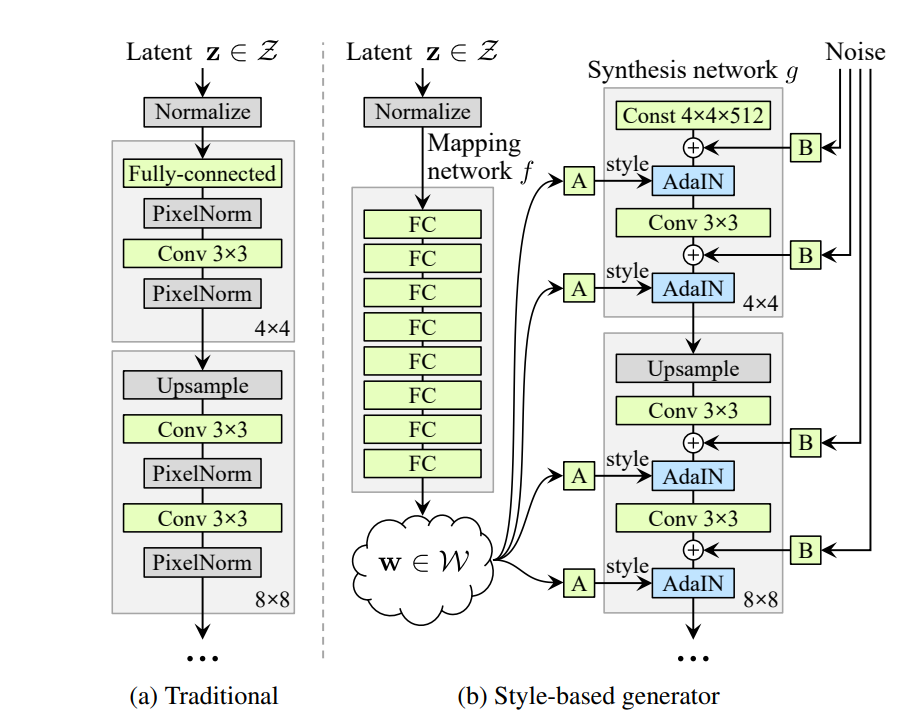
\includegraphics[width=0.8\linewidth]{styleganarchitecture.png}
        \caption{Style GAN Architecture}
    \end{figure} 
    \subsection{Baseline Progressive GAN}
    The StyleGAN generator and discriminator models are trained using the progressive growing GAN training method. This means that both models start with small images, in this case, 4×4 images. The models are fit until stable, then both discriminator and generator are expanded to double the width and height (quadruple the area), e.g. 8×8. A new block is added to each model to support the larger image size, which is faded in slowly over training. Once faded-in, the models are again trained until reasonably stable and the process is repeated with ever-larger image sizes until the desired target image size is met, such as 1024×1024.
    
    \subsection{Bilinear Sampling}
    The progressive growing GAN uses nearest neighbor layers for upsampling instead of transpose convolutional layers that are common in other generator models. The first point of deviation in the StyleGAN is that bilinear upsampling layers are unused instead of nearest neighbor.

    \subsection{Mapping Network and AdaIN}
    Next, a standalone mapping network is used that takes a randomly sampled point from the latent space as input and generates a style vector. The mapping network is comprised of eight fully connected layers. The style vector is then transformed and incorporated into each block of the generator model after the convolutional layers via an operation called adaptive instance normalization or AdaIN. The AdaIN layers involve first standardizing the output of feature map to a standard Gaussian, then adding the style vector as a bias term. The addition of the new mapping network to the architecture also results in the renaming of the generator model to a “synthesis network.”

    
    \subsection{Addition of Noise}
    The output of each convolutional layer in the synthesis network is a block of activation maps. Gaussian noise is added to each of these activation maps prior to the AdaIN operations. A different sample of noise is generated for each block and is interpreted using per-layer scaling factors. This noise is used to introduce style-level variation at a given level of detail.


    \subsection{Mixing regularization}
    Mixing regularization involves first generating two style vectors from the mapping network. A split point in the synthesis network is chosen and all AdaIN operations prior to the split point use the first style vector and all AdaIN operations after the split point get the second style vector. This encourages the layers and blocks to localize the style to specific parts of the model and corresponding level of detail in the generated image.




\end{onehalfspace}

